\documentclass[a4paper,10pt,
headsepline,           % Linie zw. Kopfzeile und Text
oneside,               % einseitig
pointlessnumbers,      % keine Punkte nach den letzten Ziffern in Überschriften
bibtotoc,              % LV im IV
DIV=15,               % Satzspiegel auf 15er Raster, schmalere Ränder   
%BCOR15mm               % Bindekorrektur
%,draft
]{scrbook}
\KOMAoptions{DIV=last} % Neuberechnung Satzspiegel nach Laden von Paket helvet


\usepackage{enumitem}

% Setzt den Abstand zwischen den Items kleiner
\setlist[itemize]{itemsep=1pt, topsep=1pt}

\pagestyle{headings}
\usepackage{blindtext}
\usepackage{multicol}
\usepackage[most]{tcolorbox} % Paket für farbige Boxen
\usepackage{xcolor} % Erweiterte Farboptionen

% Farben definieren
\definecolor{uulmlogoblue}{HTML}{89a2b3}
\definecolor{uulmblue}{HTML}{7D9AAA}
\definecolor{uulmaccent}{HTML}{A9A28D}
\definecolor{uulmgreen}{HTML}{56AA1C}
\definecolor{uulmred}{HTML}{A32638}
\definecolor{uulmorange}{HTML}{DF6D07}
\definecolor{uulmblue2}{HTML}{26547C}
\definecolor{darkgreen}{rgb}{0.0, 0.5, 0.0}

\colorlet{uulmtext}{black}
\colorlet{uulmbackground}{white}
\colorlet{uulmboxmix}{white}

% Stil für farbige Boxen mit Titel
\tcbset{
    uulm@boxstyle/.style n args=3{
        colframe=#3!50!white,
        colback=#3!20!white,
        coltitle=black,
        fonttitle=\bfseries,
        before upper={\parskip=0pt\relax},
        left=1mm, right=1mm, top=1mm, bottom=1mm,
        enhanced, boxrule=1pt, rounded corners,
        title=#2  % <-- Hier wird der Titel korrekt eingesetzt
    }
}

% Boxen für Definition, Beispiel und Notiz mit UULM Farben
\newtcolorbox{definition}[2][]{uulm@boxstyle={#1}{#2}{uulmorange}}
\newtcolorbox{example}[2][]{uulm@boxstyle={#1}{#2}{uulmblue2}}
\newtcolorbox{note}[2][]{uulm@boxstyle={#1}{#2}{uulmred}}


% für Texte in deutscher Sprache
\usepackage[ngerman]{babel}
\usepackage[utf8]{inputenc}
\usepackage[T1]{fontenc}
\usepackage{multicol}

% Helvetica als Standard-Dokumentschrift
\usepackage[scaled]{helvet}
\renewcommand{\familydefault}{\sfdefault} 

\usepackage{graphicx}

% Literaturverzeichnis mit BibLaTeX
\usepackage[babel,german=quotes]{csquotes}
\usepackage[backend=bibtex8]{biblatex}
\bibliography{bibliography}

% Für Tabellen mit fester Gesamtbreite und variabler Spaltenbreite
\usepackage{tabularx} 

% Besondere Schriftauszeichnungen
\usepackage{url}              % \url{http://...} in Schreibmaschinenschrift
\usepackage{color}            % zum Setzen farbigen Textes

\usepackage{amssymb, amsmath} % Pakete für Mathe-Umgebungen und -Symbole

\usepackage{setspace}         % Paket für div. Abstände, z.B. ZA
%\onehalfspacing              % nur dann, wenn gefordert; ist sehr groß!!
\setlength{\parindent}{0pt}   % kein linker Einzug der ersten Absatzzeile
\setlength{\parskip}{1.4ex plus 0.35ex minus 0.3ex} % Absatzabstand, leicht variabel

% Tiefe, bis zu der Überschriften in das Inhaltsverzeichnis kommen
\setcounter{tocdepth}{3}      % ist Standard

% Beispiele für Quellcode
\usepackage{listings}
\lstset{language=Python,
  showstringspaces=false,
  frame=single,
  numbers=left,
  basicstyle=\ttfamily,
  numberstyle=\tiny}

% hier Namen etc. einsetzen
\newcommand{\titel}{Fachdidaktik Physik 3 -- Handout} 
\renewcommand{\subtitle}{Textanalyse von Simple-Club-Videos}
\newcommand{\jahr}{2025}




% hier die Fakultät auswählen
%\newcommand{\fakultaet}{---  Im Quellcode anpassen nicht vergessen! ---}
\newcommand{\gremium}{Fachdidaktik Physik 3}
%\newcommand{\fakultaet}{Mathematik und\\Wirtschafts-\\wissenschaften}
%\newcommand{\fakultaet}{Medizin}
%\newcommand{\fakultaet}{Naturwissenschaften}

% Informationen, die LaTeX in die PDF-Datei schreibt
\pdfinfo{
  /Author (Matthias Ruf)
  /Title (\titel)
  /Producer     (pdfeTex 3.14159-1.30.6-2.2)
  /Keywords (project)
}

\newcommand{\co}{%
  \leavevmode
  \begingroup
  \setbox 2 = \hbox {\small c}%
  \setbox 0 = \hbox {/}%
  \dimen 0 = \ht 0  \advance \dimen 0 by -\ht 2
  \raise \dimen 0 \box 2
  \kern -0.3333\wd0/\kern -0.3333\wd 0
  \lower \dp 0 \hbox {\small o}%
  \endgroup
}

\usepackage{hyperref}
\hypersetup{
pdftitle=\titel,
pdfauthor={Matthias Ruf und Rebecca Mombrei},
pdfsubject={Positionspapier},
pdfproducer={pdfeTex 3.14159-1.30.6-2.2},
colorlinks=false,
pdfborder=0 0 0	% keine Box um die Links!
}

% Trennungsregeln
\hyphenation{Sil-ben-trenn-ung}

\begin{document}
\frontmatter

% Titelseite
\thispagestyle{empty}
\begin{addmargin*}[8mm]{8mm}

\hfill \parbox{0.23\textwidth}{
\includegraphics[width=0.23\textwidth]{./images/logo_uulm.png} }\\[4em]

\end{addmargin*}

\parbox{125mm}{\bfseries \LARGE \titel}\\[1.5em]
{\footnotesize \subtitle }\\

% ab hier Zeilenabstand etwas größer 
\setstretch{0.8}

\renewcommand{\mainmatter}{\pagenumbering{arabic}}
\mainmatter

\section*{Lesbarkeitsindex}
\begin{definition}{Theorie -- Wiener Sachtextformeln und Flesch-Index}
\textbf{Wiener Sachtextformeln:}
\begin{itemize}
    \item Berechnung der Lesbarkeit von Texten
    \item Skala von 4-15, gibt Klassen bzw. Schwierigkeitsstufe an.
\end{itemize}
            \begin{align*}
                \textbf{Formel 1}: & \quad G_1 = 0.1935 \cdot MS + 0.1672 \cdot SL + 0.1297 \cdot IW - 0.0327 \cdot ES - 0.875 \\
                \textbf{Formel 2}: & \quad G_2 = 0.2007 \cdot MS + 0.1682 \cdot SL + 0.1373 \cdot IW - 2.779 \\
                \textbf{Formel 3}: & \quad G_3 = 0.2963 \cdot MS + 0.1905 \cdot SL - 1.1144 \\
                \textbf{Formel 4}: & \quad G_4 = 0.2744 \cdot MS + 0.2656 \cdot SL - 1.693
            \end{align*}



      {\scriptsize  \textbf{MS}: Wörter mit $\geq $ 3 Silben (in \%),
        \textbf{SL}: $\varnothing $ Satzlänge (Wörter/Satz),
        \textbf{IW}: Wörter mit $>$ 6 Buchstaben,
        \textbf{ES}: einsilbige Wörter (in \%)}
\ \\[0.25em]
\textbf{Flesch-Index:}
\begin{itemize}
    \item Berechnung der Lesbarkeit von (deutschen) Texten.
    \item Skala von 100-0; je höher der Wert, desto leichter der Text.
\end{itemize}
\begin{align*}
    \textbf{Formel}: & \quad \text{FRE}_{\text{deutsch}} = 180 - SL - (58{,}8 \cdot SW)
\end{align*}
{\scriptsize \textbf{SL} = $\varnothing $ Satzlänge (Wörter/Satz), \textbf{SW} = $\varnothing $ Silbenanzahl pro Wort (Silben/Wort)}
\end{definition}

\section*{The Simple Club-Videos:}




\begin{example}{Analyse -- Lesbarkeitsindex: \glqq The Simple Club\grqq{}-Videos}
    Analysye von vier Videos zu den Newtonschen Axiomen.
    \begin{center}

		\begin{tabular}{|l|c|c|l|c|}
			\hline
			\textbf{Video} & \textbf{WSTF4} & \textbf{FRE}$_{\mathrm{de}}$ & \textbf{Video ID} & Länge (min) \\
			\hline
Newtonsche Axiome & 5.14 & 70.28  & \href{https://www.youtube.com/watch?v=skFzB2nmMwM}{skFzB2nmMwM} & 2.55 \\
			\hline
Trägheitsprinzip  & 4.35     & 72.27 & \href{https://www.youtube.com/watch?v=x04Qgfqo7Bg}{x04Qgfqo7Bg} & 4.50 \\
			\hline
Aktionsprinzip    & 4.92 & 72.42  & \href{https://www.youtube.com/watch?v=g1LfwG2pSs4}{g1LfwG2pSs4} & 5.05 \\
			\hline
Wechselwirkungsprinzip & 5.27 & 67.41  & \href{https://www.youtube.com/watch?v=TiPeS6QaEeM}{TiPeS6QaEeM} & 5.03  \\
			\hline
			\hline
\textbf{Mittelwert} & 4.92  & 70.60 & & 4.38 \\
			\hline
		\end{tabular}
	\end{center}

\begin{itemize}
		\item Mittelwert der Lesbarkeitsindex: 4.92 $\Rightarrow$ für Schüler:innen ab Klasse 5 geeignet
		\item im Bildungsplan: Gymnasium, Klasse 7/8 (und 9/10)
		\item Videos von The Simple Club zeichnen sich durch einfache Sprache aus.
	\end{itemize}

\end{example}

	

\newpage
\section*{Vergleich: Videos vs. Schulbuchtext}

\begin{multicols}{2}

\begin{example}{The Simple Club: Wechselwirkungsprinzip} 
    {\tiny \href{https://www.youtube.com/watch?v=TiPeS6QaEeM}{https://www.youtube.com/watch?v=TiPeS6QaEeM}} \\[0.5em]
    
    \begin{tabular}{lrl}
        Sätze:  & 13  & \\
        Wörter: & 172 & (13.23 pro Satz) \\
        Silben: & 284 & (1.65 pro Wort) \\
        Silben $\geq 3$:& 21 & (\textcolor{darkgreen}{\textbf{12.21\%}}) \\
        4 WSTF: & \textcolor{darkgreen}{\textbf{4.45}}  & (Klassenstufe 5)\\
        Flesch-Index: & 69.68 & (mittel verständlich)\\  
    \end{tabular}
\end{example}
    \columnbreak
    
    \begin{example}{Universum Physik: Wechselwirk. \& Gleichgew.} 
    {\tiny Universum Physik BW 9/10 (S. 234)}\\[0.5em]
    
    \begin{tabular}{lrl}
        Sätze: & 7    & \\
        Wörter: & 99  & (14.14 pro Satz) \\
        Silben: & 173 & (1.74 pro Wort) \\
        Silben $\geq 3$: & 19 & (\textcolor{red}{\textbf{19.19\%}}) \\
        4 WSTF: & \textcolor{red}{\textbf{6.69}} & (Klassenstufe 7)\\
        Flesch-Index: & 63.10 & (mittel verständlich)\\  
    \end{tabular}
\end{example}
    \end{multicols}

\begin{example}{Analysye -- Vergleich: The Simple Club vs. Schulbuchtext}
    In meinem Beispiel:
    \begin{itemize}
        \item Anteil der Wörter mit drei oder mehr Silben deutlich geringer.
        \item Einfluss von Satzlänge auf Differenz aufgrund geringer Unterschiede eher gering
        \item The Simple Club Text deutlich länger als Schulbuchtext.
        \item The Simple Club: Klassenstufe 5, Schulbuch: Klassenstufe 7
    \end{itemize}
\end{example}


    \section*{Video-Analyse-Tool}

\begin{note}{Tool -- Video Analyse Tool}
Zur Analyse der Texte wurde ein selbst entwickeltes Tool verwendet. \\[0.5em]
\begin{itemize}
    \item Tool zur Analyse von Videos:
    \begin{itemize}
        \item Texttranskription (nicht ausgereift)
        \item Berechnung des Lesbarkeitsindex (WSTF, Flesch-Index)
    \end{itemize}
    \item Code unter \url{https://github.com/LoRaMint/lesbarkeitsindex-analyser}
\end{itemize}

\begin{center}
\vspace{0.5cm}
    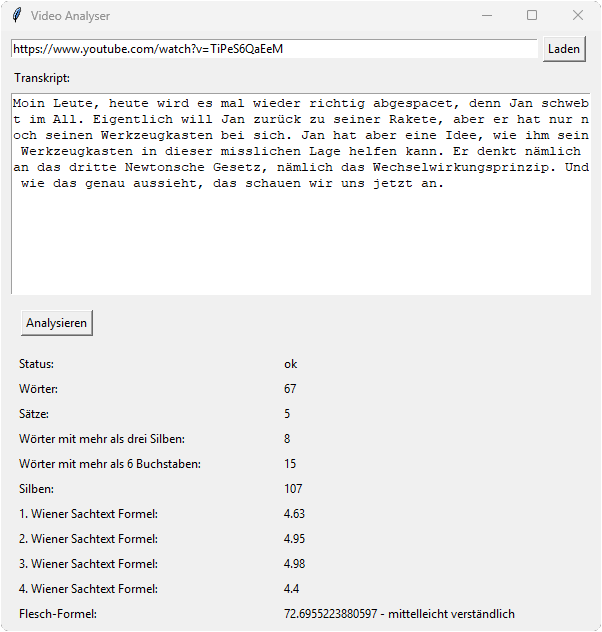
\includegraphics[width=0.4\linewidth]{images/tool.png}
    \vspace{0.25cm}

    \textbf{Abbildung:} Video-Analyse-Tool

\end{center}

\end{note}









\appendix
% hier Anhänge einbinden


\backmatter


 

\end{document}